\documentclass[border=10pt]{standalone}

\usepackage{tikz}
\usepackage{tikzsymbols}
\usetikzlibrary{calc,patterns,shapes.geometric}

\def\centerarc[#1](#2)(#3:#4:#5){\draw[#1] ($(#2)+({#5*cos(#3)},{#5*sin(#3)})$) arc (#3:#4:#5);}

\begin{document}
	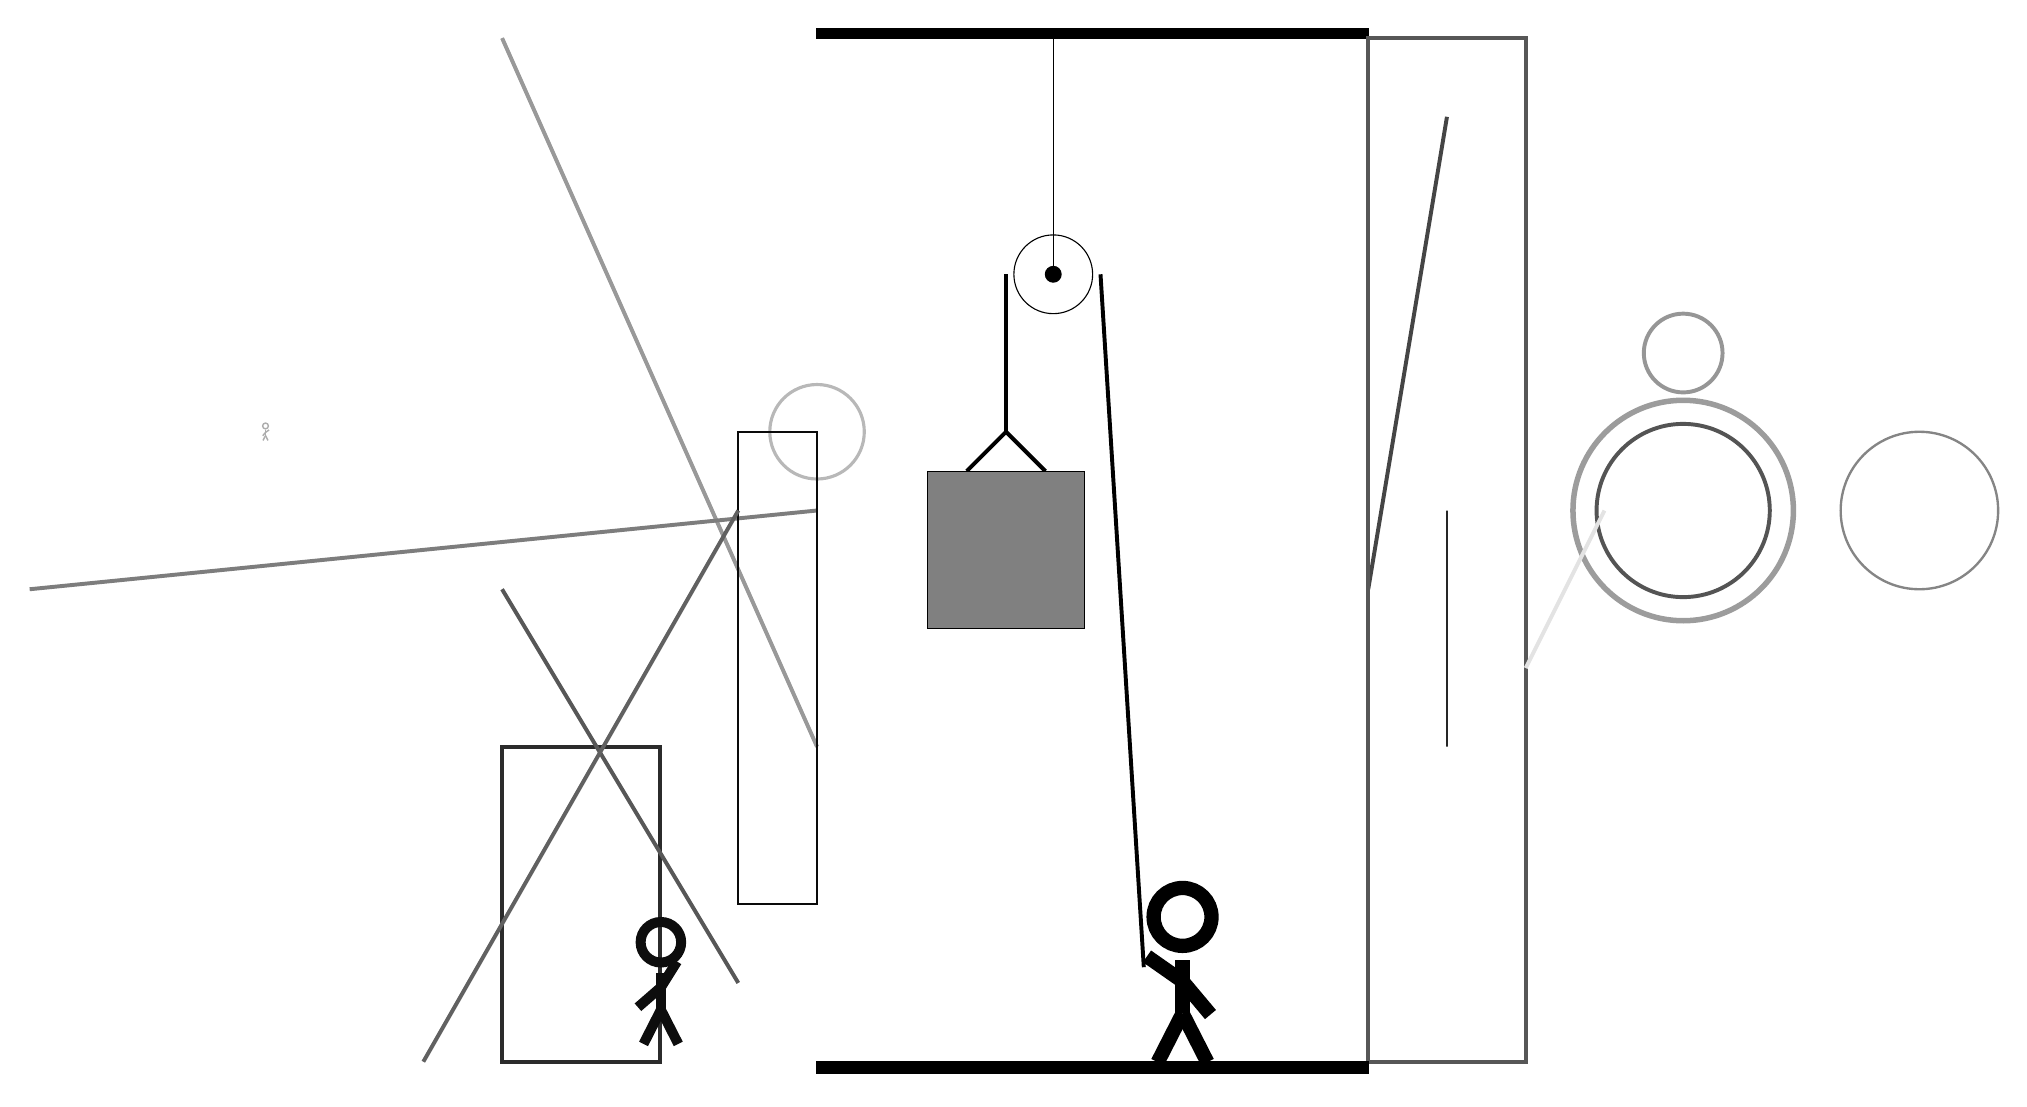
\begin{tikzpicture}
		%%%%% START %%%%%
		
		\draw[fill=black] (-2, 10) rectangle (5, 10.125);
		
		\draw (1, 7) circle (0.5);
		\draw[fill=black] (1, 7) circle (0.1);
		\draw (1, 10) -- (1, 7);
		
		\draw[line width=0.5mm] (-0.1, 4.5) -- (0.4, 5.0) -- (0.9, 4.5);
		\draw[fill=black!50] (-0.6, 4.5) rectangle (1.4, 2.5);
		
		\draw[line width=0.5mm] (0.4, 7) -- (0.4, 5.0);
		\centerarc[line width=0.5mm](1, 7)(0:180:0.6);
		\draw[line width=0.5mm](1.6, 7) -- (2.15, -1.8);
		
		\draw[line width=0.5mm, color=black!40](-2, 1) -- (-6, 10);
		
		\draw[line width=0.5mm, color=black!83] (-4, -3) rectangle (-6, 1);
		\draw[line width=0.5mm, color=black!66](-6, 3) -- (-3, -2);
		\draw[line width=0.5mm, color=black!51](-2, 4) -- (-12, 3);
		
		\draw [line width=0.4mm, color=black!28](-2, 5) circle (0.6);
		\draw [line width=0.3mm, color=black!48](12, 4) circle (1.0);
		
		\draw [line width=0.7mm, color=black!39](9, 4) circle (1.4);
		
		\draw[line width=0.5mm, color=black!73](5, 3) -- (6, 9);
		\draw[line width=0.5mm, color=black!66] (5, -3) rectangle (7, 10);
		\node[line width=0.4mm, color=black!32] at (-9, 5) {\Strichmaxerl[1][51][34]};
		\draw[line width=0.3mm, color=black!96] (-3, -1) rectangle (-2, 5);
		\draw [line width=0.5mm, color=black!41](9, 6) circle (0.5);
		\draw[line width=0.3mm, color=black!85] (6, 4) rectangle (6, 1);
		\draw[line width=0.5mm, color=black!62](-3, 4) -- (-7, -3);
		\draw[line width=0.3mm, color=black!57] (-2, -1) rectangle (-2, -1);
		\draw [line width=0.5mm, color=black!67](9, 4) circle (1.1);
		\node[line width=0.3mm, color=black!95] at (-4, -2) {\Strichmaxerl[7][41][58]};
		\draw[line width=0.5mm, color=black!11](8, 4) -- (7, 2);
		
		\node at (2.6, -1.9) {\Strichmaxerl[10][-35][-50]};
		
		\draw[fill=black] (-2, -3) rectangle (5, -3.15);
		
		%%%%% END %%%%%
	\end{tikzpicture}
\end{document}